\chapter{Project Plan}
\label{ch:plan}
This chapter covers the progress made so far, and the remaining tasks needed to be done. Figure \ref{fig:Gantt} shows the gantt chart of our project. Diamonds with orange color are milestones of the project.

\section{Progress}
The first phase of our project is carried out smoothly, followings are progress we made so far:
\begin{enumerate}
    \item Literature review: we searched and read more than 40 papaer related to our project, have a basic sense of which techniques may be required in this Project.
    \item Data collection: we searched and downloaded a stock price dataset called \textbf{Huge Stock Market Dataset}, which contains full historical daily price and volume data for all US-based stocks and ETFs trading on the NYSE, NASDAQ, and NYSE MKT.
    \item POP writing: we wrote the POP based on the marking scheme.
    \item Tool selection: we decided to use Python as the main programming language since it has various data structures that are easy to manipulate. 
    \item Code implementation (partial): we wrote some sketch of functions that will be used in our implementation.
\end{enumerate}

\section{Future Work}
Generally, the remaining tasks of this project include:
\begin{enumerate}
    \item Completion of code implementation, including (1) select proper algorithms; (2) decide programming language and libraries that will be used in this project; (3) add or re-implement functions based on our requirements; (4) design experiment methods and implement functions for evaluation.
    \item Experiment and evaluation, including (1) fed data to our models and record the output; (2) visualize the output; (3) evaluate the experimental results based on pre-defined metrics.
    \item Dissertation writing.
\end{enumerate}

\begin{figure}[!htbp]
    \centering
    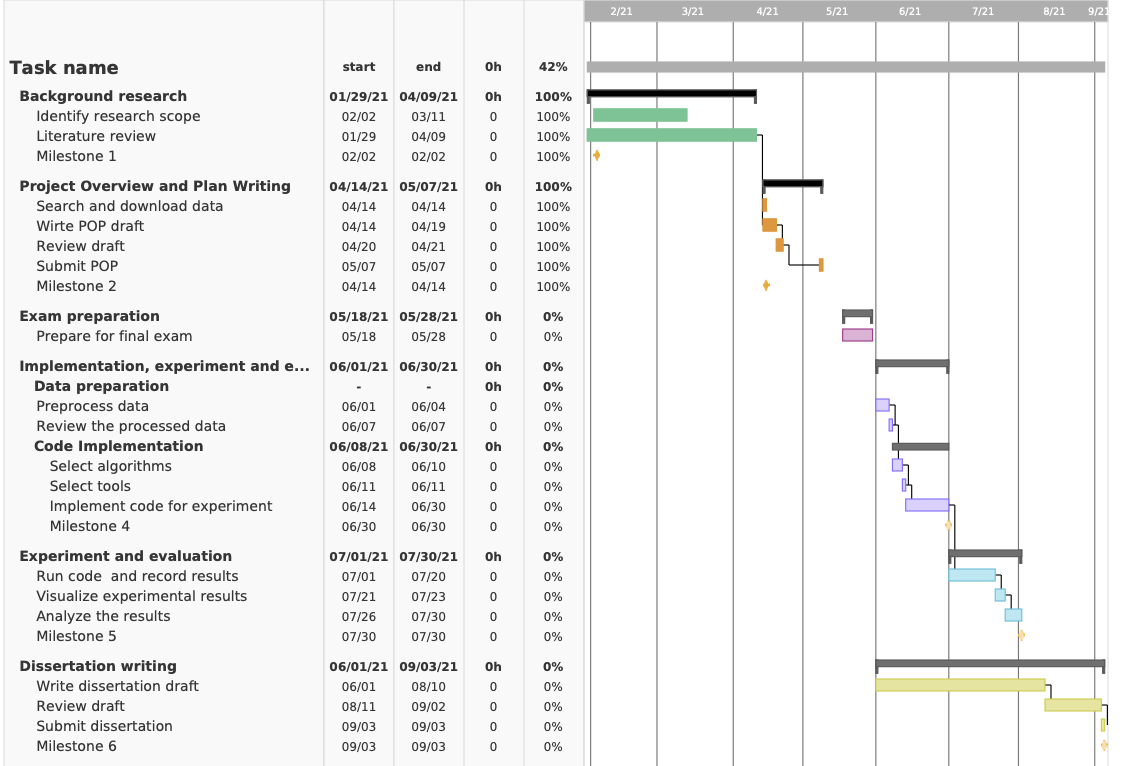
\includegraphics[width=6.5in]{schedule.png}
    \caption{Gantt Chart}
    \label{fig:Gantt}
\end{figure} 